\documentclass[a4paper, 11pt]{report}

\usepackage{lmodern}
\usepackage[french]{babel}
\usepackage[utf8]{inputenc}
\usepackage[T1]{fontenc}

\usepackage{graphicx} % Pour les images
\graphicspath{Figures}
\usepackage{caption}
\usepackage{subcaption}
\usepackage{amsmath, amsfonts, amssymb} %Pour les maths

\usepackage{textcase}

\usepackage{afterpage}

% La numérotation

\makeatletter\@addtoreset{section}{chapter}\makeatother
\renewcommand{\thepart}{\Roman{part}}
\renewcommand{\thechapter}{\arabic{chapter}}
\renewcommand{\thesection}{\Roman{section}}

\usepackage{chngcntr}
\counterwithin{figure}{section}

% Sommaire + hyperliens

\usepackage[hyphens]{url}
\usepackage[pdfauthor = {{Baptiste Braun-Delvoye}, {Julien Sagnes}}, pdftitle = {{Rapport de Projet}}, pdfstartview = Fit, pdfpagelayout = SinglePage, pdfnewwindow = true, bookmarksnumbered = true, breaklinks, colorlinks, linkcolor = black, urlcolor = black, citecolor = black, linktoc = all]{hyperref}
\usepackage[
    left = \flqq{},% 
    right = \frqq{},% 
    leftsub = \flq{},% 
    rightsub = \frq{} %
]{dirtytalk} % permet de citer mieux

% Codes

\usepackage{listings}
\usepackage{xcolor}
\usepackage[section]{placeins}
\usepackage{enumitem}
\usepackage{accsupp}

\newcommand{\noncopynumber}[1]{%
    \BeginAccSupp{method=escape,ActualText={}}%
    #1%
    \EndAccSupp{}%
}

\definecolor{codegreen}{rgb}{0,0.6,0}
\definecolor{codegray}{rgb}{0.5,0.5,0.5}
\definecolor{codepurple}{rgb}{0.58,0,0.82}
\definecolor{backcolour}{rgb}{0.95,0.95,0.92}

\lstdefinestyle{mystyle}{
    backgroundcolor=\color{backcolour},   
    commentstyle=\color{codegreen},
    keywordstyle=\color{magenta},
    numberstyle=\tiny\color{codegray},
    stringstyle=\color{codepurple},
    basicstyle=\ttfamily\footnotesize,
    breakatwhitespace=false,         
    breaklines=true,                 
    captionpos=b,                    
    keepspaces=true,                 
    numbers = left,
    numberstyle=\tiny\noncopynumber,
    numbersep=5pt,                  
    showspaces=false,                
    showstringspaces=false,
    showtabs=false,                  
    tabsize=2,
    literate=
  {á}{{\'a}}1 {é}{{\'e}}1 {í}{{\'i}}1 {ó}{{\'o}}1 {ú}{{\'u}}1
  {Á}{{\'A}}1 {É}{{\'E}}1 {Í}{{\'I}}1 {Ó}{{\'O}}1 {Ú}{{\'U}}1
  {à}{{\`a}}1 {è}{{\`e}}1 {ì}{{\`i}}1 {ò}{{\`o}}1 {ù}{{\`u}}1
  {À}{{\`A}}1 {È}{{\'E}}1 {Ì}{{\`I}}1 {Ò}{{\`O}}1 {Ù}{{\`U}}1
  {ä}{{\"a}}1 {ë}{{\"e}}1 {ï}{{\"i}}1 {ö}{{\"o}}1 {ü}{{\"u}}1
  {Ä}{{\"A}}1 {Ë}{{\"E}}1 {Ï}{{\"I}}1 {Ö}{{\"O}}1 {Ü}{{\"U}}1
  {â}{{\^a}}1 {ê}{{\^e}}1 {î}{{\^i}}1 {ô}{{\^o}}1 {û}{{\^u}}1
  {Â}{{\^A}}1 {Ê}{{\^E}}1 {Î}{{\^I}}1 {Ô}{{\^O}}1 {Û}{{\^U}}1
  {œ}{{\oe}}1 {Œ}{{\OE}}1 {æ}{{\ae}}1 {Æ}{{\AE}}1 {ß}{{\ss}}1
  {ű}{{\H{u}}}1 {Ű}{{\H{U}}}1 {ő}{{\H{o}}}1 {Ő}{{\H{O}}}1
  {ç}{{\c c}}1 {Ç}{{\c C}}1 {ø}{{\o}}1 {å}{{\r a}}1 {Å}{{\r A}}1
  {€}{{\EUR}}1 {£}{{\pounds}}1
}
\lstset{style=mystyle}
  
% Bibliographie

\usepackage{csquotes}
\usepackage[backend=biber,
style=ieee,
sorting=none
]{biblatex}
\addbibresource{biblio.bib}

% \title{Rapport Stage Pantographe Haptique}
% \author{Baptiste Braun-Delvoye, Axel Gricourt}
% \date{October 2023}

\begin{document}

\definecolor{darkWhite}{rgb}{0.94,0.94,0.94}

% Page de garde

\begin{titlepage}
    \newcommand{\HRule}{\rule{\linewidth}{0.5mm}}
    \begin{center}
        \begin{minipage}{1\linewidth}
            \begin{flushleft}
                \hspace{4.5cm}
                
\includegraphics[width=0.25\textwidth]{Figures/SORBONNE_FAC_SCIENCES_DEF_CMJN.pdf}
            \end{flushleft}
        \end{minipage}

        \vspace{1.5cm}
        
        \textsc{\Large{}Master SAR 1\up{\MakeTextLowercase{ère}} année} \\[0.5cm]
        \textsc{\large{}2024 - 2025} \\[0.5cm]

        \HRule \\[0.6cm]
        {\huge\bfseries{}Rapport de Projet de Modélisation :} \\ \LARGE{Conception, Modélisation et Commande d'un robot parallèle 3RRR} \\[0.25cm]
        \HRule \\[1.5cm]


        \Large\textit{Auteurs :}\\
        \begin{center}
            Baptiste \textsc{Braun-Delvoye}\\
            Julien \textsc{Sagnes}
        \end{center}

        \hfill

        \Large\textit{Professeur :}\\
        \begin{center}
            Faiz \textsc{Ben-Amar}
        \end{center}
        \vspace{1cm}
        {\large\today} \\[2cm]
    \end{center}

    \vfill
\end{titlepage}


\selectlanguage{french} 
% \addcontentsline{toc}{section}{Abstract}

\clearpage\setcounter{page}{2}

\tableofcontents

\section*{Introduction}
\addcontentsline{toc}{section}{Introduction}

\section{Conception}

Pour la conception, nous utilisons le logiciel SolidWorks. Nous avons décidé de suivre le modèle du TP pour dessiner les différentes pièces, en s'assurant de garder des distances de l'ordre de la dizaine de centimètre ; il est question de ne pas faire un robot trop grand.

\subsection{Bras du robot}

Dans un premier temps, nous concevons les bras qui composent le robot pour décider de la taille générale de la maquette.
Également, il est question de minimiser la quantité de matériaux utilisée pour les différentes pièces dans l'objectif de réduire le coût d'impression 3D.
Nous opérons donc une optimisation topologique sur les différents bras en effectuant des allègements, comme nous pouvons le voir sur la figure \ref{fig:bras}, 
qui détaille aussi les côtes des pièces en millimètres. Du reste, nous utilisons des congés pour adoucir les bords des pièces afin de rendre le robot plus harmonieux.

\begin{figure}[h]
    \centering
    \begin{subfigure}[t]{0.55\textwidth}
        \centering
        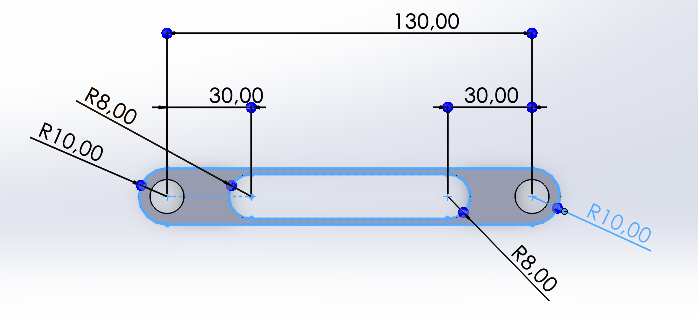
\includegraphics[width=\textwidth]{Figures/bras_effecteur.png}
        \caption{Bras effecteur}
        \label{fig:bras_effecteur}
    \end{subfigure}
    \hfill
    \begin{subfigure}[t]{0.40\textwidth}
        \centering
        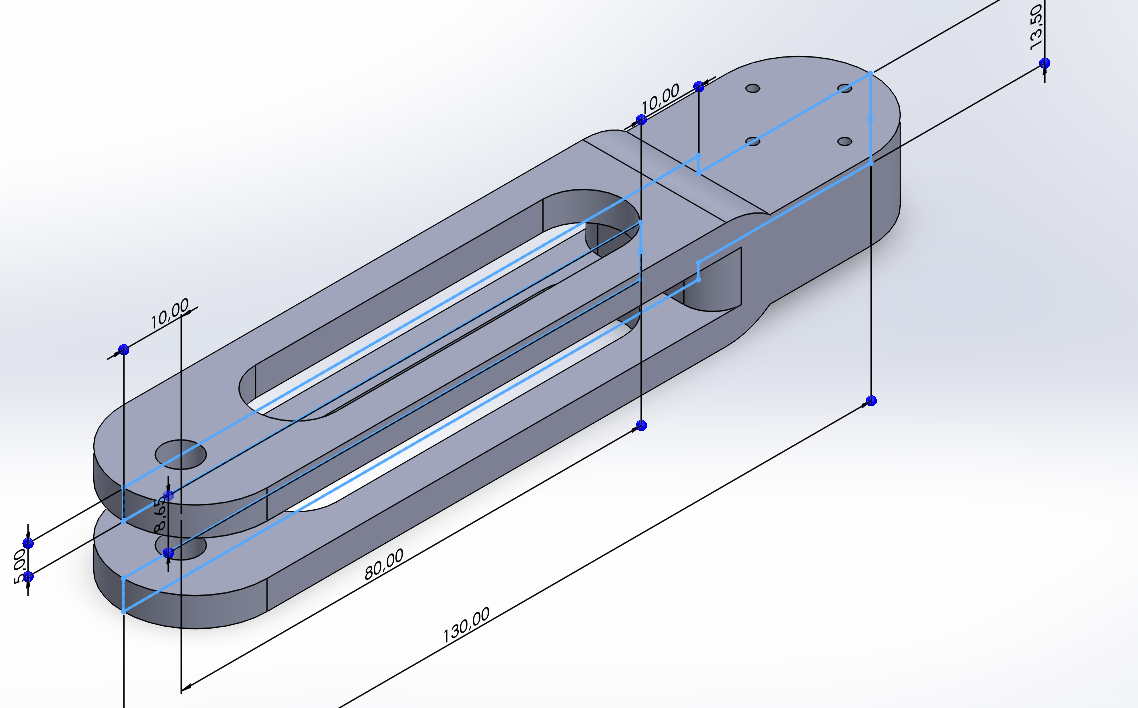
\includegraphics[width=\textwidth]{Figures/bras_moteur.png}
        \caption{Bras moteur}
        \label{fig:bras_moteur}
    \end{subfigure}
    \caption{Allègement des bras du robot}
    \label{fig:bras}
\end{figure}

\subsection{Effecteur}

Pour l'effecteur, nous optons pour une forme triangulaire, dont les côtés sont agencés de telle sorte qu'ils puissent auceuillir les boulons.
En effet, les trous que nous faisons sur les pièces ont pour but d'acceuillir des boulons M6 (diamètre du trou 6.3 mm), auquel on rajoute un jeu de 0.15 mm.

\section{Simulation}

\section{Réalisation}

\section*{Conclusion}
\addcontentsline{toc}{section}{Conclusion}

% \newpage

% \newpage
% \nocite{*}
% \addcontentsline{toc}{section}{Bibliographie} 
% \printbibliography
\end{document}